\chapter{Introduction}

Welcome to \textit{Linux Filesystems -- Under the Cover}, the first book dedicated to Linux filesystems in over 20 years but only the first book dedicated to Linux filesystem internals.

The first book that I could find was \textit{Linux Filesystems} by William Von Hagen \cite{hagen}, a book that, to be honest, I didn't know existed until I searched while writing this section. Unlike Von Hagen's book, this book goes very deep into the Linux kernel virtual filesystem implementation as well as the implementation of several popular filesystems.

This book also follows on from my second book \textit{UNIX Filesystems -- Evolution, Design and Implementation} \cite{pate-filesystems} that was published in 2003. It's hard to think that was now 20 years ago! That book covered filesystems across many versions of UNIX, microkernel-based implementations of UNIX and also Linux, just as it was moving to the 2.4 kernel series. At the time, my team at VERITAS had just finished porting the VERITAS filesystem VxFS. VxFS was a filesystem that ran on SVR4 UNIX variants, Solaris, HP-UX, AIX and Linux.

In 2004 I VERITAS left to start working on a series of books on the Linux kernel. I set a lofty goal of trying to do for Linux what Donald Knuth had done for computer algorithms. I didn't get very far getting pulled back into corporate America and spending the next twenty years working in various startups, two of my own. I was quite surprised in 2022 when I came back to book writing to discover that there still wasn't a great deal of information on Linux filesystems and very few Linux kernel books had been published in many years. There are some great articles on the web but they are spread across many different sites, quite sparse in specific areas and are often quite dated.

And thus begins my journey one more time. The kernel has become too vast to try the Donald Knuth approach so I decided to focus on filesystems, the part of the kernel I've worked on and been most interested in for over thirty years now. Even with a focus on filesystems there is a lot of material and throughout the process, I've gone back and forth on whether this should be one or two volumes. Passing the 400 page mark with a vast amount of material still to cover, I decided that it should be two volumes which was my original goal. The first volume focuses and generic filesystem implementation while the second goes into detail on specific filesystems and covers the more unusual aspects of filesystem access.

I still wanted to focus on the practical side of things so there are lots of examples given using a variety of different tools and example filesystems in both the kernel and user-space. To support the book I'm providing course materials that you can find online and my own website with blog material and more detailed examples.

I hope you enjoy reading the book as much as I've enjoyed writing it.

%%%%%%%%%%%%%%%%%%%%%%%%%%%%%%%%%%%%%%%%%%%%%%%%%%%%%%%%%%%%%%%%%

\section{About me}

Despite writing an interpreter in 6502 assembler at High School and wanting to work in \textit{systems programming}, my first introduction to operating systems kernel came in 1985 when one of the instructors at Leeds University (in the UK) gave an informal walkthrough of the 3BSD kernel source code. At this time, the BSD source code could be found on every system under \cf{/sys}. I believe that the machine we were using was a DEC PDP-11. It was also around this time that Kernighan and Ritchie’s "\textit{The C Programming Language}" \cite{kernighan} was one of the few books available about C. If you wanted to learn about UNIX, Kernighan and Pike’s "\textit{The UNIX Programming Environment}" \cite{pike} was the book of choice having just been launched the year I started college. Both are now available free on-line.

I was lucky to work on the Chorus Microkernel early during my career while I was at ICL (International Computers Limited), the UK’s largest mainframe manufacturer, later acquired by Fujitsu. After working on European research projects based around Chorus, we started enhancing the SVR4 UNIX subsystem running on top of the microkernel to make it production ready for a Sparc-based distributed server we planned to ship. This involved porting the VERITAS filesystem (VxFS) and volume manager (VxVM) from vanilla SVR4 UNIX. I worked on the latter. Due to the very different interactions between filesystems and the virtual memory (VM) subsystems of both Chorus MiX (their version of SVR4) and standard SVR4 UNIX, the port of the filesystem was an arduous task. The volume manager less so (lucky for me). Over those years I gained an insight into the operations of different kernel implementations and my love of filesystems started. 

In 1993 I joined SCO (Santa Cruz Operation) partly to help them to switch over from an SVR3 UNIX Filesystem Switch (FSS) architecture to support the Sun/USL VFS/vnode based architecture. As was ICL, we were looking to modernize our filesystem support and bring in support for newer filesystems such as VxFS which were light years ahead of anything on most UNIX variants at that time. Two things prevented that move. First, the cost of rewriting large parts of the kernel were prohibitive. Secondly, the cost of converting existing filesystems over to a new VFS/vnode architecture would also add significant expense. And on top of that, SCO acquired the rights to UNIX which then gave them SVR4 UNIX (and therefore "vnodes") anyway.

I led the SCO kernel architecture team whose job it was to look at more forward thinking features, new architectures like the upcoming RISC-based Intel P6 which was abandoned following their agreement with HP. We also started investigating a new microkernel-based architecture of UNIX to replace existing European telecom companies proprietary operating systems.

While running the architecture team, I wrote my first book covering SCO OpenServer UNIX internals \cite{pate-unix}, which was at that time, a much enhanced version of SVR3. We’d abandoned the idea of SVR4 VFS/vnodes but had implemented support for a journaling filesystem from an east coast US company called Prologic. We also completely rewrote the virtual memory subsystem to support \cf{mmap(2)} and therefore support of the SVR4 development environment (compiler etc). Much of that work was done by Hugh Dickens who went on to make many contributions to the Linux kernel and is still working on Linux for Google as I write.

\begin{wrapfigure}{L}{0.3\textwidth}
	\centering
	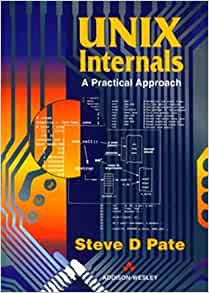
\includegraphics[scale=0.4]{figures/book-1.jpg}
\end{wrapfigure}

To explain how things have become more complicated over the decades, in 1996, I was very happy to get my hands on Lyon's book "\textit{A Commentary on the UNIX Operating System}" \cite{lions}. This described the 6th Edition UNIX kernel which was less than 9,000 LOC (Lines Of Code). At that time, I was working on porting the \cf{truss(1)} command (UNIX equivalent of \cf{strace(1)}) over to the Chorus microkernel. The \cf{truss} command itself was around 10,000 LOC.

I was proud of this first book. It’s not easy to write about a proprietary operating system but it started my journey in writing in as practical a way as possible to better help people understand the subject matter. The book had many programming examples and use of the \cf{crash(1)} command to display the contents of kernel structures after user-space commands are run and system calls are made. I've followed a similar approach in this book.

I continued working on the Chorus microkernel as part of a consortium between SCO, Chorus and Siemens Private Networks. At first this was an SVR3-based UNIX subsystem running on Chorus but that was switched to SVR4.2 MP (multi-processing). Once again we started porting VxFS and VxVM over to the microkernel but made better choices to largely emulate SVR4 interfaces to simplify the port. And then SCO abandoned the project and started spiraling downwards as a company. I left the UK in 1996 and joined VERITAS to work in Mountain View, California. It was interesting, but at that time, SGI were building all around the area north of Shoreline. Years later, the vast majority of their buildings were taken over by Google and that's still where Google's headquarters is today.

As a side note, SCO used to hold its annual SCO Forum each summer at UC Santa Cruz. The summer before leaving SCO, I pulled together a panel session to discuss the future of operating systems and managed to get Bill Shannon (Sun employee 11), Michel Gien (co-founder of Chorus Systemes), someone representing the Mach microkernel whose name escapes me and Linus Torvalds. Linus was still living in Finland at the time so we flew him over to California to spend the week with us. Unfortunately I have no photos of the event. Linus's view was that the future of operating systems was the desktop. Perhaps that wasn't the right answer but at that time, who knew the future of server operating systems would be dominated by Linux? After searching to see where people still were, I was saddened to see that Bill Shannon died in 2020. You can read about him here:

\begin{table}[h]
\begin{tabular}{lcl}
\parbox[r]{0.5in}{
\includegraphics[scale=0.15]{figures/url.png}} & \parbox[l]{0.55in}{URL \arabic{urls} -- } & \parbox[l]{3in}{\cf{https://tinyurl.com/4j9j496n}}
\end{tabular}
\end{table}
\stepcounter{urls}
% https://blog.dshr.org/2020/06/bill-shannon-rip.html

\noindent
As an operating system enthusiast, the VERITAS filesystem was a great place to work. The VERITAS filesystem VxFS ran on a number of different operating systems. I initially started working on the portability project where we tried to share as much code as possible on UnixWare, HP-UX and Solaris. Later on we added AIX and I ran the team that ported VxFS to Linux. 

While at VERITAS I wrote my second book. This one covered filesystems from a variety of different UNIX and UNIX-like operating systems. I included a sample Linux filesystem similar to the kernel-based filesystem presented in this book. At the time, this was for the 2.4.x kernel and a lot has changed since then.

\begin{wrapfigure}{L}{0.4\textwidth}
	\centering
	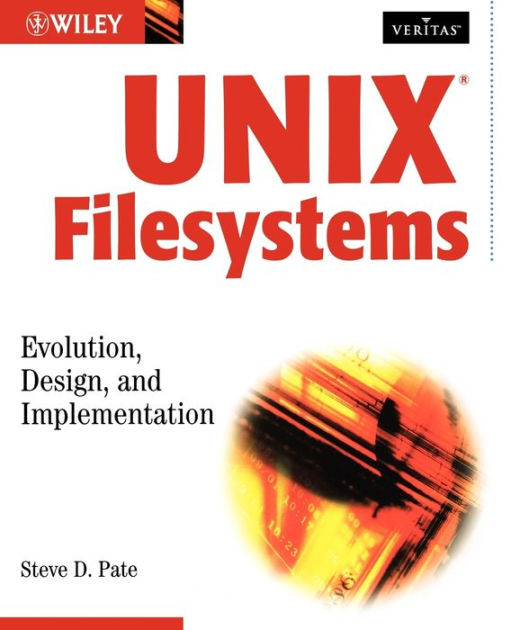
\includegraphics[scale=0.8]{figures/book-2.jpg}
\end{wrapfigure}

Being in Silicon Valley, I was surrounded by startups and went to work for two unsuccessful storage companies. At the second we actually engaged with Hans Reiser to enhance ReieserFS. I shudder at the thought! I then moved to work for Vormetric, initially consulting on their cross-platform encryption filesystem product and then  later as CTO. They were an enterprise encryption and key management company that encrypted at both the filesystem and volume layers, also for a wide array of operating systems (Solaris, AIX, HP-UX, Linux and Windows). I then spent the next 14 years working on virtualization security and encryption and key management technologies in the two startups I co-founded, HyTrust and HighCloud Security. Both involved encrypting at the filesystem and device driver layer on both FreeBSD and Linux. As a strange twist of events, HyTrust acquired HighCloud in 2012. I stayed with HyTrust for 5 years post-acquisition before moving to Thales (who acquired Vormetric) where I worked with several old friends helping with the merger of Thales and Gemalto encryption technologies.

That brings us to the present day and back to book writing but now full time. I looked to see what material was out there about Linux filesystems and surprised to see that there was a gap that needed to be filled. And thus, I started coding again for the first time in years (apart from writing Space Invaders in Python/pygame) with the goal to build simple filesystems that are easy to explain and play with. They are all included on this book and github with additional examples on my website.

This book is allowing me to achieve something I've wanted to do for many years and that is to write it and typeset it using \LaTeX which I have used for many years. I actually typeset my first two books. My first book was written using Microsoft Word which actually worked fine but struggled with such a large number of pages. I was disappointed with FrameMaker when typesetting my second book. The program just didn't seem as simple and easy to use as it did when I used the early versions of FrameMaker on my old Sun Sparcstation 1. 

Book writing is a lot of work for little financial gain. My last two books didn't exactly make me rich! This time around I intend to self-publish so I can hopefully more money especially given that I am now writing books and educational material as a full-time job. It will also be quite a learning curve to understand the book industry beyond just writing and typesetting. It's a path I started back in 2014 with help from my first editor at Addison Wesley, Karen Mosman. It's only taken 19 years to finally get there.

%%%%%%%%%%%%%%%%%%%%%%%%%%%%%%%%%%%%%%%%%%%%%%%%%%%%%%%%%%%%%%%%%

\section{Isn't Everything Documented On-line?}

The short answer is no. The longer answer is that some aspects of the kernel's filesystem-independent and filesystem-dependent code is documented and there is quite a lot of detailed information available on very specific topics. For example, some of the nitty gritty details around pathname resolution are documented, specifically around fast paths and locking. But even with this level of detail, the high-level picture of pathname resolution and with figures and examples, are very hard to come by.

I had no intention of cutting and pasting text from online and I think that too much detail isn't worth it in many areas. If you get the big picture, you can then go further to get the details. Or perhaps the big picture is enough for your goals. Where I have taken material from on-line, I reference the material and often, I'll tell you to read the on-line documentation to go further. I'll also be writing blog posts to pull things together further \textbf{XXX}.

%%%%%%%%%%%%%%%%%%%%%%%%%%%%%%%%%%%%%%%%%%%%%%%%%%%%%%%%%%%%%%%%%

\section{Why Isn't the Material Open Source?}

Since I'm writing about one of the largest open source projects of all time, I'm sure a lot of people will be wondering why write a book for profit and not just put the material online. My answer is quite simple. I can't afford to do that. This is the first book I'm writing while not currently employed and I need to make some money. After all, beer isn't free. My plan is to allow make on-line courses using the same material and have a web presence where I can blog, bring source code up to date and write about new filesystem changes that may make it into a future version. Perhaps one day I'll write a filesystem in Rust. Whether this can be profitable is to be seen. So in the meantime, I need to pay the bills. 

%%%%%%%%%%%%%%%%%%%%%%%%%%%%%%%%%%%%%%%%%%%%%%%%%%%%%%%%%%%%%%%%%

\section{Feedback}

Because of self-publishing, I have more control over the content and distribution of material. I can print a smaller number of books and make additional editions to expand, correct and bring material up to date. To do this, feedback is essential. You can leave feedback in the regular places (amazon.com for example), on my website ({\bfseries XXX---TBD} or by emailing me directly at spate@me.com ({\bfseries XXX---I need a work email address}).

%%%%%%%%%%%%%%%%%%%%%%%%%%%%%%%%%%%%%%%%%%%%%%%%%%%%%%%%%%%%%%%%%

\section{Do you do anything for fun?}

Credibility is important when writing a book, presenting technical information or representing your company in any formal capacity. Hopefully the information above will show that I have the knowledge and experience to write such a book. Having said that, when reading a review of my last book, one reviewer was complimentary of my book but asked whether I actually did anything for fun. I was amused and vowed that if I ever wrote another book, I'd actually add information about myself other than what I've done technically. So here goes!

\begin{wrapfigure}{L}{0.4\textwidth}
	\centering
	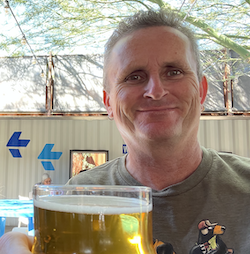
\includegraphics[scale=0.8]{figures/beer.png}
\end{wrapfigure}

I've been an avid sports fan all my life playing almost every sport you can think of in competitive capacity. This was mostly football/soccer in my early years including a short sting with Southampton Football club youth training program back in the early 80s. But I competed for the high school team in basketball, volleyball, high jump, and cross country. I run every week (several half marathons under my belt), hike the mountains around Tucson, Arizona, do yoga and cycle a lot. When I turned 50, I completed 50 rides of 50+ miles including 2 centuries, 3 metric centuries and a lot of rides between 50-55 miles. At the time I'm writing this we just finished the Tour de Tucson metric century. Not bad for a vegan of 36 years!

\noindent
My favorite teams are Newcastle United, San Francisco Giants, San Francisco 49ers, Golden State Warriors and the Oregon Ducks (my daughter went to college there).

Oh and I'm a great fan of beer, growing up with Newcastle Brown Ale and British Bitters but having developed more of a taste for IPAs over the last several years. On a cold winter's night (yes, we do get some in Arizona) I love a big, heavy imperial stout (or two).

%%%%%%%%%%%%%%%%%%%%%%%%%%%%%%%%%%%%%%%%%%%%%%%%%%%%%%%%%%%%%%%%%

\section{Conventions}

I try to follow man page sections when commands, libraries and system calls are referenced. So \cf{umount(1)} refers to the \cf{umount} command while \cf{umount(2)} refers to the system call. If \cf{umount} is used without a section reference it refers more to one or the other but generally just during the time when the filesystem is being unmounted.

Internal functions such as those used by the SPFS disk-based filesystem are shown without a manpage reference. An example would be \cf{sp\_read\_inode()}. The same is true for Linux kernel variables and functions.

There are a few commands that are also used as verbs such as \cf{grep} which will be shown in courier font but without the manpage number.

Processes run in either user-space or kernel-space. Some times these are referred to as user space and kernel space, or in the latter case just \textit{in the kernel}. I refer to them as user-space and kernel-space.

Finally, there are a few peculiarities to point out. It's traditional in the UNIX/Linux space to say \textit{filesystems} instead of \textit{file systems}. UNIX is also written in all caps even though it is not an acronym. I had long arguments with a previous publisher over this.

%%%%%%%%%%%%%%%%%%%%%%%%%%%%%%%%%%%%%%%%%%%%%%%%%%%%%%%%%%%%%%%%%

\subsection{What Error Checking?}

Most of the example programs do little in the way of checking for errors. This is a terrible way to program but since many of the source code examples are displayed throughout the book, and are there for teaching purposes only, I've omitted most error checking to reduce the amount of code that's displayed. In the chapter on building a disk-based filesystem, there is a lot more error checking since failing to check for errors in the kernel can lead to panics. At times when displaying this code, I've omitted \cf{printk()} statements and error checking for the purpose of describing the flow more easily.

%%%%%%%%%%%%%%%%%%%%%%%%%%%%%%%%%%%%%%%%%%%%%%%%%%%%%%%%%%%%%%%%%

\subsection{Source Code References}

Where relevant we show where in the Linux source code relevant structures and functions can be found. For example, in the section that describes the kernel structures used for mounted filesystems, you will see a callout as follows:

\begin{table}[h]
\begin{tabular}{ll}
\parbox[l]{0.5in}{
\includegraphics[scale=0.8]{figures/src-xref.pdf}} & \parbox[l]{4in}{\small{\cf{fs/filesystems.c} contains the \cf{file\_systems} variable, routines to register / unregister filesystems and functions for handling \cf{struct filesystem-type} including searching for filesystems during \cf{mount(2)}.}}
\end{tabular}
\end{table}

\noindent
Pathnames are relative to the top of the Linux kernel source tree so \cf{fs/filesystems.c} will be located at \cf{linux-6.1.10/fs/filesystems.c} for example.

%%%%%%%%%%%%%%%%%%%%%%%%%%%%%%%%%%%%%%%%%%%%%%%%%%%%%%%%%%%%%%%%%

\subsection{Web References}

There are multiple times where I've given an internet URL knowing that at some point in the future the server may disappear and  the link could become invalid. I've still included the link in short-form making it easier to type. I have also added a section on my website where I will endeavor to make sure that these links are up-to-date. So if a link does become invalid, I'll include a new reference as appropriate.

Each time I give a reference you'll see it like this:

\begin{table}[h]
\begin{tabular}{lcl}
\parbox[r]{0.5in}{ 
\includegraphics[scale=0.15]{figures/url.png}} & \parbox[l]{0.1in}{2} & \parbox[l]{3in}{\cf{https://tinyurl.com/5bnxjrae}}
\end{tabular}
\end{table}
\stepcounter{urls}

\noindent
Thus if you look at the list of ordered references on my website, it will be easy to see the number and be able to click on the  link. Throughout the book I use \cf{www.tinyurl.com} to generate the URLs so it's easier for you to type them. Unless of course the URL is small enough to being with. At times, you can just search for relevant terms and you'll end up at the correct site.

%%%%%%%%%%%%%%%%%%%%%%%%%%%%%%%%%%%%%%%%%%%%%%%%%%%%%%%%%%%%%%%%%

\section{I Versus we vs ...}

It used to be very common with technical material to write in the third person. While I do that a lot of most of the time, the main goal of the material to be instructive so will use I/we/our as appropriate depending on the subject matter being discussed and whether it's more demonstration-based as opposed to a description. So although it may not be the most grammatically correct, I believe that it makes it more readable.
 
 %%%%%%%%%%%%%%%%%%%%%%%%%%%%%%%%%%%%%%%%%%%%%%%%%%%%%%%%%%%%%%%%%
 
\section{Who Should Read This Book?}

Learning to program in the kernel is not a trivial task and with the huge growth of Linux in terms of its size (over 25 million LOC), learning about the Linux kernel is more of a daunting task today that in the past. There quite is a lot of documentation on-line that didn't exist years ago but it's largely incomplete and most of the Linux kernel internals books are now largely out of date. To some degree this is understandable. Linux has continued to evolve at a fast pace supporting more and more devices from laptops to servers, from mobile phones to supercomputers. There is still a lot of interest in how filesystems work and this is one area that hasn't had a lot of coverage over the years and very little in terms of published material.

This book should appeal to anyone interested in learning more about how filesystems operate but also give the tools to be able to develop simple filesystems in both user-space and in the kernel. That's where the fun is despite being challenging. 

Readers should at least be familiar with the C programming language since the Linux kernel and all filesystems are written in C. At the time of writing, support for Rust has been announced but we're still a long way from being able to develop filesystems in Rust. Perhaps look for a blog entry on that or a newer edition of this book.

The book should appeal to undergraduate and post-graduate students who wish to pursue a career in the operating system or system programming field. It's always been the case the kernel-level engineers can work at any layer in the software stack but not necessarily the other way around. I feel that this is largely due to solid debugging skills that kernel engineers must develop often with limited tools.

%%%%%%%%%%%%%%%%%%%%%%%%%%%%%%%%%%%%%%%%%%%%%%%%%%%%%%%%%%%%%%%%%

\section{What's in the Book?}

Readers can jump around as needed of course but the book is written in a style such that each chapter builds on the prior chapter. You need to understand the programming interfaces before you start looking at the kernel. File access in particular uses many different flags resulting in a lot of "if ... then" statements in the kernel depending on which flags are set. The same is true for filesystem management. The basics are explained first before digging deep into how Linux supports them at different layers.

Once more basic concepts have been explained, the kernel source tree layout is described together with information about a set of tools that make it easy for navigating your way through the kernel sources. The location of file and filesystem structures and functions is detailed together with references to the kernel files where the structures and functions are defined.

With knowledge of how the kernel structures for file and filesystem access are linked together, the book then describes in more detail the flow through the kernel functions for supporting file and filesystem related system calls.

To help make sense of how everything works they will be an example disk-based file system which is fully functional and less than 1500 lines of source code making it easy to understand. There are also two user-based filesystems based on the FUSE infrastructure. First is a simple pass-through file system and the second encrypts file contents.

\begin{figure}[h]
	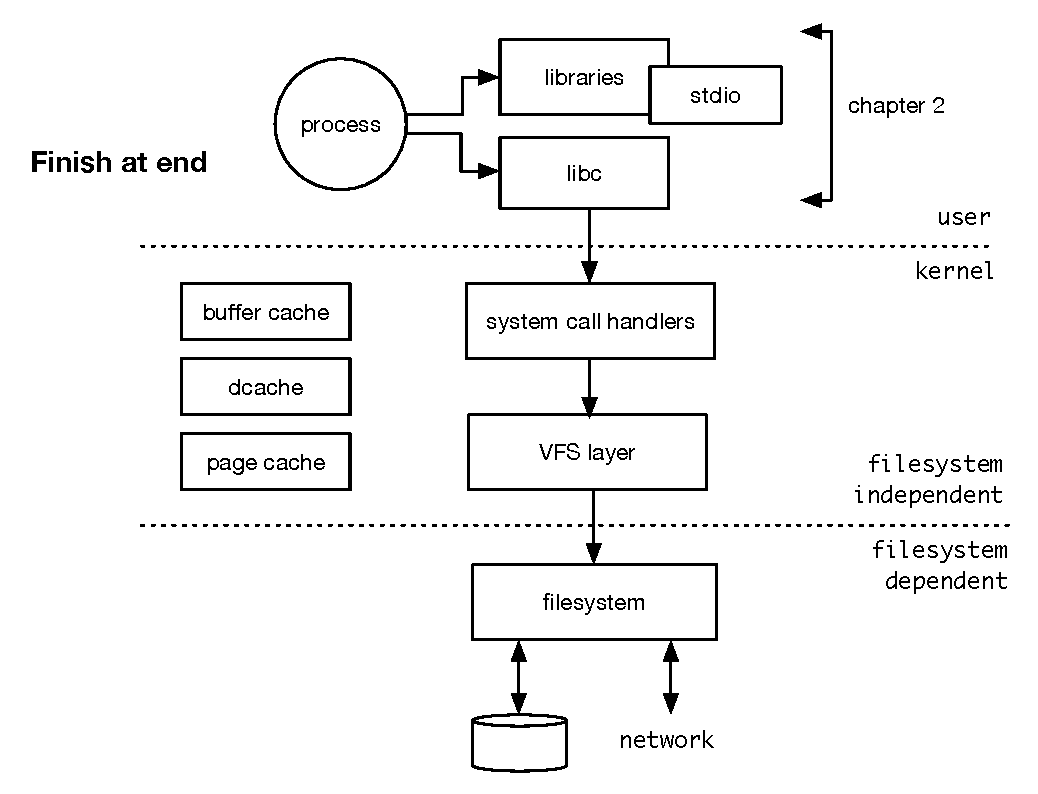
\includegraphics[scale=0.6]{figures/intro-figure.pdf}
	\centering
	\caption{Various subsystems in Linux and their location in the book}
	\label{fig:intro-figure}
\end{figure}

The book concludes with chapters on debugging techniques, file system performance and filesystem security. Figure \ref{fig:intro-figure} highlights the parts of a Linux operating system and where each is covered in the book. In more detail, here is the breakdown of each chapter:

\begin{itemize}
	\item{\textbf{Chapter 1 -- Introduction}} -- This chapter.
	\item{\textbf{Chapter 2 -- File and Filesystem Programming}} -- before understanding how the Linux kernel provides support
		for filesystems and file access, it's necessary to explore the different commands, system calls and 
		library functions that applications use to access files and filesystems. This chapter provides information
		on the Linux standards followed, manual pages (manpages), file types, programming interfaces, 
		sparse files and various types of I/O including direct I/O and asynchronous I/O. The standard I/O
		library is discussed in detail with information about how to browse the standard library source code.
		There is a section on reading directory entries with a simple implementation of the \cf{ls(1)} command.
	\item{\textbf{Chapter 3 -- Filesystems}} -- this chapter covers everything from the different file systems that 
		Linux provides to the operations that can be applied to them such as mounting, unmounting and reporting 
		disk usage. Physical and pseudo filesystems will be described together with highlights of network 
		and FUSE-based file systems including a demonstration of SSHFS which allows you to view remote 
		files as if they were mounted locally. We will also cover backup and restore, quotas, swap space and 
		how the boot process works in terms of filesystem access.
	\item{\textbf{Chapter 4 -- A First Look at the Linux Source Code}} -- with 25 million lines of source code, the 
		Linux kernel is one very large piece of code and can be daunting, especially if you've never spent much 
		or any time looking at it! The chapter describes the layout of the source code and focuses on where the
		main file and filesystem structures and routines can be found. It describes various tools that can
		be used to navigate around the source code from the simple such as \cf{vim} and tag stack to 
		the more complete solutions such as \cf{cscope(1)} and Elixir. The chapter then describes the
		main structures that related to filesystems and show how the structures are linked together. The
		main routines will be highlighted together with a few simple examples and browsing through
		kernel structures using \cf{gdb}.
	\item \textbf{Chapter 5 -- Common Linux Types} -- \textbf{TBD}
	\item \textbf{Chapter 6 -- The VFS Layer} -- Following on from the previous chapter which covered the main 
		structures related to filesystems, this chapter goes much deeper in explaining the code paths through the
		kernel functions to respond to the various filesystem related system calls.
	\item \textbf{Chapter 7 -- Filesystem Case Studies} -- \textbf{TBD}
	\item{\textbf{Chapter 8 -- Building a Kernel-based Filesystem}} -- this is a fun chapter! It presents a fully 
		functional, disk-based file system that contains less than 1500 lines of source code. The foul system was 
		developed on Ubuntu Linux but should be able to run on any version of Linux. It comes with tools 
		for making a file system and a file system debugger. Volatile system is very simple in nature it 
		does support the majority of foul system operations. For fun it also includes an undelete command.
	\item{\textbf{Chapter 9 -- The FUSE Filesystem Framework}} -- the FUSE implementation in the Linux kernel 
		allows developers to implement file systems in user a space. This chapter provides two examples for 
		FUSE, one which provides a pass-through set of operations reflecting what is under the file system on 
		which it is mounted. The second example builds on the first by providing encryption of files and file names 
		using very simple key management. The implementation of the FUSE architecture will be presented 
		together with information about performance gains that have been achieved over the years including 
		some new performance enhancements using eBPF.
	\item{\textbf{Chapter 10 -- Filesystem Debugging}} -- debugging kernel code is certainly a challenge. 
		Application developers have an array of filesystem debug us to choose from including \cf{gdb}. In my 
		career I've spent many a year debugging file system code at assembler level which can be fun but not for 
		the faint hearted. This chapter covers debugging the kernel at source level using GDP but also explores a 
		number of other different debugging techniques including the more recent and very powerful eBPF tools.
	\item{\textbf{Chapter 11 -- Filesystem Performance}} -- they have been many books written about UNIX and 
		Linux performance over the years. Although this book won't go into the detail that other books and 
		articles online have covered but this chapter will explore the main performance related aspects of 
		file access and in particular some of the new eBPF performance tools.
	\item{\textbf{Chapter 12 -- Filesystem Security}} -- security is a very large topic and there are many tools, 
		standards and practices for securing file system data. This chapter highlights the bank security concerns 
		with foul and foul system access and describes everything from standard UNIX file permissions to 
		encryption key management. Security based sub systems like SELinux and AppArmor are 
		also explored.
\end{itemize}

%%%%%%%%%%%%%%%%%%%%%%%%%%%%%%%%%%%%%%%%%%%%%%%%%%%%%%%%%%%%%%%%%

\section{Why is Source Code Missing?}

There are many examples throughout the book where I only display part of a kernel structure, part of a function or even strip down some functions to remove error checking and other parts of the function. The goal behind this is to show the most relevant structures and fields and the most prominent paths through functions. I think this is preferable to putting in large amounts of source code and making it harder to see the big picture. Just bear this in mind when browsing the kernel source.

%%%%%%%%%%%%%%%%%%%%%%%%%%%%%%%%%%%%%%%%%%%%%%%%%%%%%%%%%%%%%%%%%

\section{KGDB Demonstrations}

In various sections throughout the book you will see headings such as:

\begin{quote}
\textbf{4.2.1 KGDB --- Analyzing Per-file Kernel Structures}
\end{quote}

\noindent
In these sections, I use \cf{gdb} and the kernel source-level debugger stub \cf{kgdb} to demonstrate the subject matter being displayed. There are also online videos on my YouTube channel showing more detailed versions that I recommend you watch. All  demonstrations will help reinforce the material presented.

Generally speaking, when I demonstrate an area of the kernel using \cf{gdb} there will be an accompanying YouTube video

\begin{table}[h]
\begin{tabular}{ll}
\parbox[l]{0.6in}{
\includegraphics[scale=0.3]{figures/video-camera.pdf}} & \parbox[l]{4in}{\small{\textbf{VIDEO 2} -- Analyzing VFS structures for open files}}
\end{tabular}
\end{table}

\noindent
If you look at the list of video references on my website, it will be easy to see the number and be able to click on the link. I thought this would be easier than putting URLs in here.

Before looking through the kgdb examples, I'd recommend that you read the section \ref{kgdb} first. Even if you skip all the steps to set up kgdb, look at the command and examples to understand the process that's being followed. 

In all examples, I'm going to make use of what \cf{gdb} calls \textit{convenience variables} that reference the structures that are being analyzed. No one can remember long memory addresses and I think this is the easiest way to help with understanding the flow. It's not the quickest method and there will be scripts to help with that. \textbf{XXXX-maybe / maybe not}

%%%%%%%%%%%%%%%%%%%%%%%%%%%%%%%%%%%%%%%%%%%%%%%%%%%%%%%%%%%%%%%%%

\section{Source Code Figures}[h]

There are several different ways that source is described throughout the book. Often the code is just printed as is. Sometimes, only relevant parts of a function are described and there many times during which \cf{gdb} is used to display stack backtraces which help to understand how certain functions are reached.

I find it helpful to use a drawing package to add code fragments and arrows showing how they're all connected. I use OmniGraffle, a drawing package that I've used for many years. Figure \ref{fig:code-walkthrough} gives an example of such a figure.

\begin{figure}[h]
	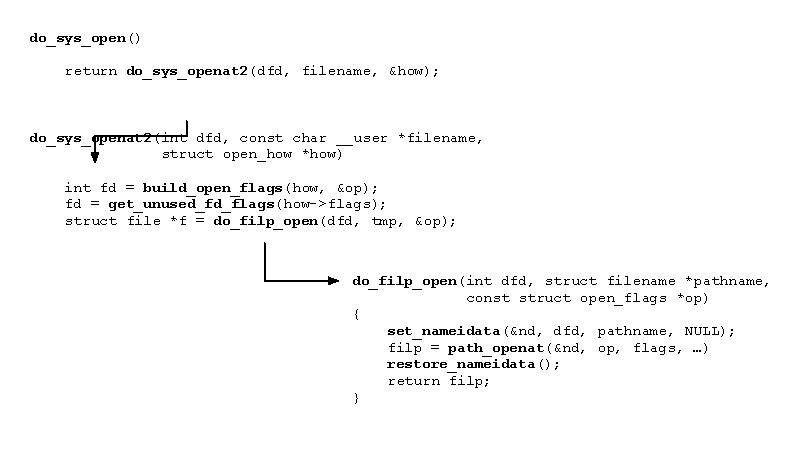
\includegraphics[scale=0.64]{figures/code-walkthrough.pdf}
	\centering
	\caption{Example Figure Showing Code Paths through the Linux Kernel}
	\label{fig:code-walkthrough}
\end{figure}

A few of these figures are shown throughout the book but rarely with this much detail. To help your understanding of how the Linux kernel works, I've collected several of these figures together. You can download them from my website -- \textbf{details TBD}

%%%%%%%%%%%%%%%%%%%%%%%%%%%%%%%%%%%%%%%%%%%%%%%%%%%%%%%%%%%%%%%%%

\section{Acknowledgements}

First and foremost, a big thank you to Eleanor who encouraged me to work on book writing full-time, which is quite a commitment. It's now almost 30 years since the publication of my first book. I've really enjoyed the process in the past but to be able to do it full time rather than cram it into evenings and weekends has made the process much more enjoyable.

Thanks to \textbf{xxx and yyy} for reviewing the material. 

Thanks to Lukas Brand who sent me an article about filesystem security. While planning the book, I forgot that I'd been in the security industry working on filesystem and device encryption for the last 15 years!

\textbf{TBD --- do this last}



